\section{案例研究:对RC4流密码的密码学分析}

RC4流密码由Ron Rivest在1987年设计,历史上曾用于保护网络流量(在SSL/TLS协议中)和无线流量(在802.11b WEP协议中)的安全。它被设计为可在内存很小的$8$位处理器上运行。虽然RC4仍在使用,但它已被证明容易遭受一些显著的攻击,因而不应该被应用在新的项目中。我们对RC4的讨论可以作为流密码分析的一个优雅的例子。

RC4密码的核心是一个PRG,称为RC4 PRG。PRG维护一个内部状态,包含一个$256$字节的数组$S$和两个额外的字节$i,j$,作为指入$S$的两个指针。数组$S$包含$\{0,\dots,255\}$中的所有的数字,且每个数字正好出现一次。图 \ref{fig:3-12} 给出了一个 RC4 状态的例子。

\begin{figure}
  \centering
  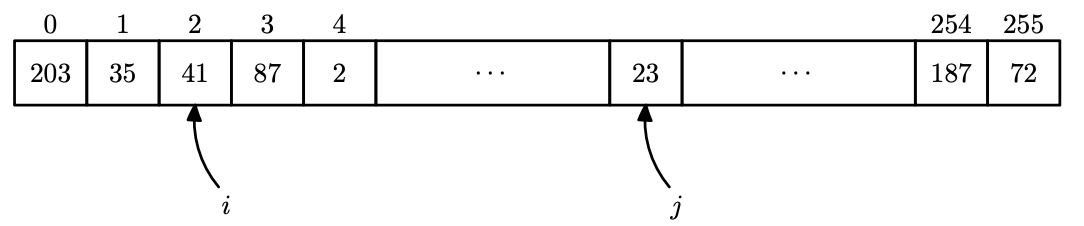
\includegraphics[width=0.75\linewidth]{figures/chapter3/fig12.png}
  \caption{RC4内部状态的一个例子}
  \label{fig:3-12}
\end{figure}

RC4流密码的密钥 $s$ 也是 PRG 的种子,用于将数组 $S$ 初始化为数字 $0 \dots 255$ 一个伪随机置换排列。初始化是使用下面的\textbf{设置算法(setup algorithm)}进行的:

\vspace*{5pt}

\hspace*{5pt} 输入:字节序列$s$

\vspace{3pt}

\hspace*{5pt} 对于 $i=1,\dots,255$:\\
\hspace*{50pt} 令 $S[i]\leftarrow i$ \\
\hspace*{26pt} 令 $j\leftarrow0$\\
\hspace*{26pt} 对于 $i=1,\dots,255$:\\
\hspace*{50pt} 令 $k\leftarrow s[i\;\mathrm{mod}\;|s|]$ \quad\quad // \emph{从种子中提取一个字节}\\
\hspace*{50pt} 令 $j\leftarrow(j+S[i]+k)\;\mathrm{mod}\;256$\\
\hspace*{50pt} $\mathrm{swap}(S[i],S[j])$

\vspace*{5pt}

在循环过程中,索引 $i$ 在数组中线性增长,而索引 $j$ 则跳来跳去。在每次迭代中,指针 $i$ 所指向的内容都会与 $j$ 所指向的内容互换。

一旦数组 $S$ 被初始化,PRG 就可以使用下面的\textbf{流生成器(stream generator)}一次生成一个字节的伪随机输出:

\vspace*{5pt}

\hspace*{5pt} 令 $i\leftarrow0$,$j\leftarrow0$\\
\hspace*{26pt} 重复:\\
\hspace*{50pt} 令 $i\leftarrow(i+1) \;\mathrm{mod}\;256$\\
\hspace*{50pt} 令 $j\leftarrow(j+S[i])\;\mathrm{mod}\;256$\\
\hspace*{50pt} $\mathrm{swap}(S[i],S[j])$ \\
\hspace*{50pt} 输出 $S\big[\,(S[i]+S[j])\;\mathrm{mod}\;256\,\big]$ \\
\hspace*{26pt} 直到永远

\vspace*{5pt}

该程序的运行时间视需要而定。同样地,索引 $i$ 在数组中线性增长,而索引 $j$ 则跳来跳去。交换 $S[i]$ 和 $S[j]$ 会不断地打乱数组 $S$。

\begin{snote}[RC4的加密速度。]
RC4 很适合用软件实现。其他流密码,如 Grain 和 Trivium,是为硬件设计的,在软件实现下的性能表现很差。表 \ref{tab:3-1} 提供了 RC4 和其他一些软件实现的流密码的运行时间对比。现代处理器运行在 $64$ 比特字长上,使得基于 $8$ 比特设计的 RC4 在这些架构上稍显缓慢。
\end{snote}

\begin{table}
  \centering
  \begin{tabular}{|c|c|}
    \hline
    密码 & 速度\footnotemark[1](MB/s)\\
    \hline
    RC4 & 126\\
    SEAL & 375\\
    Salsa20 & 408\\
    Sosemanuk & 727\\
    \hline
  \end{tabular}
  \caption{软件实现的流密码的速度比较(速度越高越好)。}
\end{table}

\subsection{RC4的安全性}

\footnotetext[1]{性能数字是使用 Crypto++ 5.6.0 benchmark 在 1.83 Ghz Intel Core 2 处理器上运行获得的。}

RC4一度被认为是一个安全的流密码,并被广泛部署在应用程序中。在一些攻击表明它的输出有一定的偏差后,该密码就失宠了。我们下面提出两种攻击,它们都能将 RC4 的输出与随机字符串区分开来。在本小节中,我们用$n$表示数组$S$的大小。对于RC4,我们有$n=256$。

\begin{snote}[初始 RC4 输出中的偏差。]
RC4的设置算法基于给定的随机种子将数组$S$初始化为$0 \dots 255$的一个置换。我们先暂且假设 RC4 的设置算法是完美的,它能从所有可能的 $256!$ 个排列组合中产生一个均匀的置换排列。Mantin和Shamir表明,即使假设初始化是完美的,RC4 的输出也是有偏差的。
\end{snote}

\begin{lemma}[Mantin-Shamir定理]\label{lemma:3-8}
假设数组 $S$ 被设置为 $0\dots n-1$ 的一个随机排列,并且 $i$ 和 $j$ 都被置为 $0$,那么 RC4 输出的第二个字节等于 $0$ 的概率为 $2/n$。
\end{lemma}

\begin{proof}[证明思路]
令$z_2$是 RC4 输出的第二个字节。令 $P$ 是 $S[2]=0$和 $S[1]\neq2$ 成立的事件。关键的观察是,当事件 $P$ 发生时,$z_2=0$ 的概率为 $1$,见图 \ref{fig:3-13}。然而,当 $P$ 没有发生时,$z_2$ 均匀分布在 $0\dots n-1$ 上,因此它等于 $0$ 的概率为 $1/n$。由于 $\Pr[P]$ 约为 $1/n$,我们可以得到以下(近似)结果:
\[
\begin{aligned}
\Pr[z_2=0] & =\Pr[(z_2=0)\;|\;P]\cdot\Pr[P]+\Pr[(z_2=0)\;|\;\neg P]\cdot\Pr[\neg P]\\
& \approx 1\cdot(1/n)+(1/n)\cdot(1-1/n)\approx2/n\qedhere
\end{aligned}
\]
\end{proof}

该引理表明,RC4输出的第二个字节为 $0$ 的概率是它本应有的两倍。这就导出了一个简单的 RC4 PRG 区分器。给定一个序列$x\in\{0,\dots,255\}^\ell$,对于$\ell\geq2$,如果$x$的第二个字节是$0$,区分器输出$0$,否则就输出$1$。根据引理 \ref{lemma:3-8},这个区分器的优势约为 $1/n$,对于 RC4 来说就是 $0.39\%$。

\begin{figure}
  \centering
  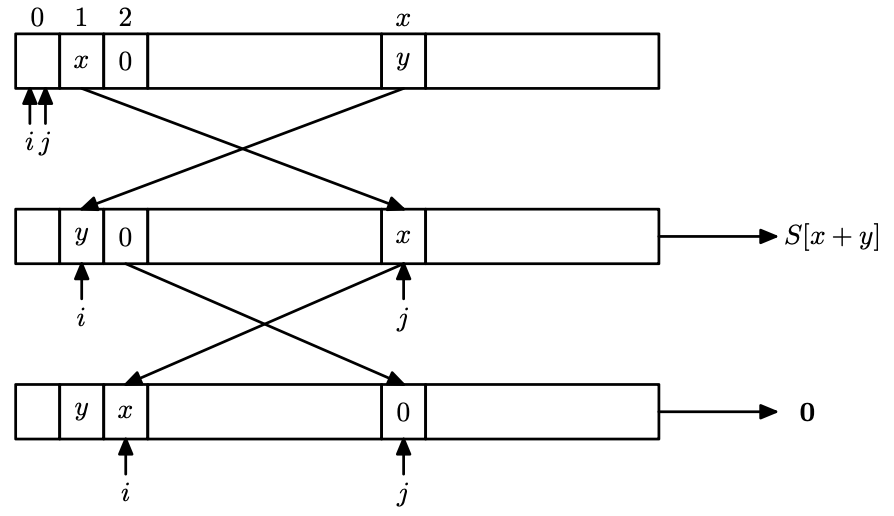
\includegraphics[width=0.55\linewidth]{figures/chapter3/fig13.png}
  \caption{引理 \ref{lemma:3-8} 的证明}
  \label{fig:3-13}
\end{figure}

Mantin-Shamir 区分器表明 RC4 输出的第二字节是有偏差的。AlFardan等人推广了这一结论,他们通过测量许多随机密钥上的偏差,表明输出的前$256$个字节中的每一个都有偏差:每个字节的分布都与均匀性相差甚远。这种偏差不像第二字节那样明显,但它仍是不可忽略不计的,足以用来对密码发动攻击。例如,他们表明,给定用 $2^{30}$ 个随机密钥加密的单一明文的对应密文,我们有可能以接近 $1$ 的概率恢复明文的前 $128$ 字节。这种攻击很容易在网络上进行,因为在网络上,一个秘密的 cookie 通常被嵌入到一个消息的前几个字节中。每次浏览器连接到受害者的网络服务器时,这个 cookie 都会用新的密钥重新加密。攻击者可以使用 Javascript 脚本令用户的浏览器反复重连到目标网站,以向攻击者提供发动攻击和暴露 cookie 所需的 $2^{30}$ 个密文。

作为回应,RSA实验室发布了一项建议,建议放弃RC4流生成器输出的前 $1024$ 字节,而只使用第 $1025$ 字节及以后的字节。这可以防御最初的密钥流偏差区分器,但不能防御我们接下来将要讨论的攻击。

\begin{snote}[RC4流生成器中的偏差。]
假设RC4设置算法已经被修改,从而使得上面介绍的攻击无效。Fluhrer和McGrew给出了一个直接针对流生成器的攻击。他们声称字节对$(0,0)$ 在 RC4 的输出中出现的次数多于它应该在随机序列中出现的次数。这足以将 RC4 的输出与随序列区分开来。

令 $\mathrm{ST}_\mathrm{RC4}$ 为 RC4 所有可能的内部状态的集合。由于数组 $S$ 有 $n$ 个可能的设置,$i$ 和 $j$ 各有 $n$ 个可能的设置,所以 $\mathrm{ST}_\mathrm{RC4}$ 的大小为 $n!\cdot n^2$。由于在 RC4 中$n=256$,$\mathrm{ST}_\mathrm{RC4}$ 的大小是非常巨大的,大约为 $10^{511}$。
\end{snote}

\begin{lemma}[Fluhrer-McGrew定理]
假设RC4使用一个$\mathrm{ST}_\mathrm{RC4}$中的随机状态$T$初始化。令$(z_1,z_2)$是 RC4 在状态 $T$ 下启动时输出的前两个字节。则有:
\[
\begin{aligned}\label{lemma:3-9}
& i\neq n−1 & \Longrightarrow & \quad\Pr[(z_1,z_2)=(0,0)]\geq(1/n^2)\cdot\big(1+(1/n)\big)\\
& i\neq 0,1 & \Longrightarrow & \quad\Pr[(z_1,z_2)=(0,1)]\geq(1/n^2)\cdot\big(1+(1/n)\big)
\end{aligned}
\]
\end{lemma}

我们将一对连续输出 $(z_1,z_2)$ 称为一个\textbf{二重字(digraph)}。在一个真正的随机序列中,所有二重字$(x,y)$出现的概率都应当正好是 $1/n^2$。上面的引理表明,对于RC4,$(0,0)$出现的概率比它应有的值大$1/n^3$。$(0,1)$也是如此。事实上,除了引理 \ref{lemma:3-9} 所述的两个二重字,Fluhrer-McGrew 还确定了其他几个异常的二重字。

该引理导出了一个简单的区分 RC4 的输出和随机序列的区分器 $D$。如果区分器在给定的序列中发现的 $(0,0)$ 的数量大于随机序列中应有的数量,它就输出 $1$,否则就输出 $0$。

\vspace*{5pt}

\hspace*{5pt} 输入:序列$s\in\{0,\dots,n\}^\ell$\\
\hspace*{26pt} 输出:$0$ 或 $1$

\vspace{3pt}

\hspace*{5pt} 令 $q$ 为 $x$ 中出现二重字 $(0,0)$ 的次数\\
\hspace*{26pt} 如果 $(q/\ell)-(1/n^2)>1/(2n^3)$ 则输出 $0$,否则输出 $1$

\vspace*{5pt}

使用定理 \ref{theo:B-3},我们可以估计出 $D$ 的优势与输入长度 $\ell$ 的关系。特别地,区分器 $D$ 能获取下述优势:
\[
\begin{aligned}
\ell=2^{14}\text{ 字节}: &\quad\quad \mathrm{PRG}\mathsf{adv}[D,RC4]\geq2^{-8}\\
\ell=2^{34}\text{ 字节}: &\quad\quad \mathrm{PRG}\mathsf{adv}[D,RC4]\geq0.5
\end{aligned}
\]
使用Fluhrer和McGrew提供的所有异常二重字,我们就可以建立一个区分器,只用 $2^{30.6}$ 字节的输出就能实现 $0.8$ 的优势。

\begin{snote}[对RC4的相关密钥攻击。]
Fluhrer、Mantin和Shamir表明,RC4 与相关密钥一起使用时是不安全的。我们将在 \ref{sec:9-10} 节的攻击 $2$ 中讨论这种攻击及其对 802.11b WiFi 协议的影响。
\end{snote}






















































